\documentclass[12pt, a4paper]{report}
\usepackage[utf8]{inputenc}
\newcommand\preamble{
    \usepackage[italian]{babel}
    \usepackage{geometry}
    \usepackage{amsmath}
    \usepackage{amssymb}
    \usepackage{graphicx}
    \usepackage{ulem}
    \geometry{margin=2cm}
    \usepackage{listings}
    \let\olditemize\itemize
    \renewcommand\itemize{\olditemize\setlength\itemsep{0em}}
}
% Definizione delle variabili
\newcommand{\imagePath}{Immagini/logoUni.png}

% Definizione del comando per la pagina di titolo con argomenti
\newcommand{\customTitlePage}[5]{
    \newcommand{\courseTitle}{#1}
    \newcommand{\authorName}{#2}
    \newcommand{\academicYear}{#3}
    \newcommand{\universityName}{#4}
    
    \begin{titlepage}
        \centering
        \includegraphics[width=0.5\textwidth]{\imagePath}\par\vspace{1cm}
        {\scshape\LARGE \universityName \par}
        \vspace{1.5cm}
        {\huge\bfseries \courseTitle \par}
        \vspace{2cm}
        {\Large\itshape \authorName \par}
        \vfill
        \academicYear
    \end{titlepage}
}

\preamble

\begin{document}
\customTitlePage{Fondamenti di Computazione Quantistica}{Lorenzo Vaccarecci}{Anno Accademico 2024/2025}{Università degli Studi di Genova}
\newpage
\tableofcontents
\chapter{Introduzione}
\section{Porte logiche universali}
\begin{itemize}
    \item \texttt{NOT(A)} $\equiv \bar{A}$
    \item \texttt{AND(A,B)} $\equiv A \cdot B$ oppure $A \land B$
    \item \texttt{OR(A,B)} $\equiv A + B$ oppure $A \lor B$
    \item \texttt{XOR(A,B)} $\equiv A \oplus B = (A+B) \mod 2$
    \item \texttt{NAND(A,B)} $\equiv \bar{A \cdot B}$ oppure $\bar{A \lor B}$
    \item \texttt{NOR(A,B)} $\equiv \bar{A + B}$ oppure $\bar{A \land B}$
\end{itemize}
L'insieme di \texttt{AND} e \texttt{NOT} oppure di \texttt{OR} e \texttt{NOT} sono insiemi universali. Questo significa che, ad esempio, usando solo combinazioni di porte \texttt{AND} e \texttt{NOT} è possibile implementare una qualsiasi funzione booleana. Pur formando set universali, le porte \texttt{AND}, \texttt{OR}, \texttt{NAND} e \texttt{NOR} sono però \textbf{irreversibili}. A livello concettuale è interessante introdurre delle porte logiche che siano \textbf{reversibili}. Questo vuol dire che se combiniamo in sequenza una porta logica reversibile con la sua inversa, riotteniamo l'informazione originale. La porta di Fredkin può essere interpretata come uno \textit{switch} controllato di bit. Il bit di controllo è \texttt{A}; se questo è acceso i bit \texttt{B} e \texttt{C} vengono scambiati, altrimenti vengono lasciati identici.
\begin{center}
    \begin{tabular}{|c|c|c|c|c|c|}
    \hline
    \texttt{A} & \texttt{B} & \texttt{C} & \texttt{Out1} & \texttt{Out2} & \texttt{Out3} \\
    \hline
    0 & 0 & 0 & 0 & 0 & 0 \\
    \hline
    0 & 0 & 1 & 0 & 0 & 1 \\
    \hline
    0 & 1 & 0 & 0 & 1 & 0 \\
    \hline
    0 & 1 & 1 & 0 & 1 & 1 \\
    \hline
    1 & 0 & 0 & 1 & 0 & 0 \\
    \hline
    1 & 0 & 1 & 1 & 1 & 0 \\
    \hline
    1 & 1 & 0 & 1 & 0 & 1 \\
    \hline
    1 & 1 & 1 & 1 & 1 & 1 \\
    \hline
    \end{tabular}
    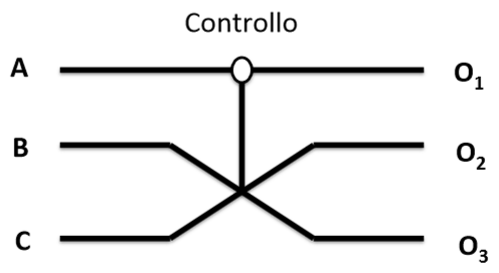
\includegraphics[width=0.4\textwidth]{Immagini/fredkin_circuit.png}
\end{center}
\section{Operazioni Bit-a-Bit}
A una stringa di $n$ bit possiamo associare un intero compreso fra 0 e $N-1$ con $N=2^n$. All'intero $x$ associamo la stringa di bit $x_0x_1x_2\dots x_{n}$ con $x_{i}=0,1 \text{ e } i=0,1,\dots,n$ tale che $x=\sum_{i=0}^{n}x_{i}2^{n-i}$. Possiamo codificare $N=2^{n}$ interi ma questi saranno compresi fra 0 e $N-1=2^{n}-1$.
\subsection{Prodotto interno bit-per-bit}
\begin{equation*}
    x\cdot z \equiv (x_{1}z_{1} + x_{2}z_{2} + \dots + x_{n}z_{n}) \mod 2
\end{equation*}
E' anche chiamato prodotto \texttt{AND} bitwise perchè si ottiene prendendo le operazioni \texttt{AND} fra i singoli bit.
\subsection{Somma bit-per-bit: bitwise \texttt{XOR}}
Indichiamo con $x\oplus z$ la somma bit-per bit, modulo 2. Il risultato questa volta è una stringa il cui $i$-esimo bit ha il valore $x_{i}+z_{i} \mod 2 = x_{i} \text{ \texttt{XOR} } z_{i}$.
\section{Prerequisiti matematici}
\subsection{Numeri complessi}
Ogni numero complesso $z\in \mathbb{C}$ può essere scritto come $z=a+ib$, con $a\in \mathbb{R}$ \textbf{parte reale} e $b\in \mathbb{R}$ \textbf{parte immaginaria}. Se $z=a+ib$ e $w=c+id$, abbiamo
\begin{equation*}
    z+w = (a+c) + i(b+d)
\end{equation*}
\begin{equation*}
    z\cdot w = (ac-bd) + i(ad+bc)
\end{equation*}
Per ogni $z\in \mathbb{C}$, $z\cdot z^{*}=a^{2}+b^{2}$ è reale e non negativo dove $z^{*}$ è il \textbf{complesso coniugato} di $z$ (la parte complessa è negata). Inoltre, $\sqrt{a^{2}+b^{2}}=\lvert z\rvert$ è detto \textbf{modulo} di $z$.
\begin{equation*}
    \lvert z\rvert^{2} = z\cdot z^{*}
\end{equation*}
Possiamo rappresentare un numero complesso $z=a+ib$ come una coppia (a,b) sul piano complesso. L'asse delle ascisse è utilizzato per la parte reale e l'asse delle ordinate per la parte immaginaria. Si ha $a = \lvert z \rvert \cos \theta$ e $b = \lvert z \rvert \sin \theta$ dove $\theta$ è la \textbf{fase}. Se $z=0$ allora $\theta$ non è definita. Per $\lvert z \rvert = 1, z=\cos\theta + i\sin\theta$. Più in generale possiamo scrivere $z=pe^{i\theta}$ con $p=\lvert z \rvert$ e $e^{i\theta}=\cos\theta + i\sin\theta$.
\subsection{Spazi vettoriali in 2D}
\begin{itemize}
    \item \textbf{Direzione}: rappresentata dalla retta su cui giace il vettore
    \item \textbf{Verso}:  specifica in che direzione punta il vettore
\end{itemize}
Se abbiamo due vettori $u$ e $v$ possiamo definire la somma che sarà un vettore $w=u+v$ ottenuto mediante la \textbf{regola del parallelogramma}.\\
Dato un numero $\alpha\in \mathbb{R}$, per ogni vettore $v$, possiamo definire il vettore $\alpha v$ è la freccia ottenuta moltiplicando $v$ per $\alpha$ in modulo e lasciando invariata la direzione se $\alpha > 0$ e invertendo il verso se $\alpha < 0$. Questa operazione è detta \textbf{moltiplicazione per scalare}. Se $\alpha = -1$, otteniamo il vettore $-v$ che ha stesso modulo, stessa direzione ma verso opposto a $v$.\\
L'insieme di tutti i vettori del piano è allora uno spazio vettoriale reale $V$ chiuso rispetto all'operazione di combinazione lineare:
\begin{equation*}
    u = \alpha v + \beta w
\end{equation*}
Per ogni vettore $u$ e $v \in V$ e per ogni $\alpha, \beta \in \mathbb{R}$.
\subsection{Prodotto scalare e componenti}
\begin{equation*}
    < \cdot, \cdot > : V \times V \rightarrow \mathbb{C}
\end{equation*}
Che soddisfa le seguenti proprietà:
\begin{enumerate}
    \item $\forall u\in V, <u,u>$ è un numero reale non negativo, con $<u,u>=0 \iff u=0$
    \item $\forall u,v \in V, <u,v>=<v,u>^{*}$
    \item $\forall u,v,w \in V,\forall \alpha,\beta \in \mathbb{C}, <w,\alpha u+\beta v>=\alpha<w,u>+\beta<w,v>$
\end{enumerate}
Due vettori per i quali il prodotto scalare è nullo sono \textit{ortogonali}, sono base ortogonali se sono ortogonali e a norma unitaria ($\lVert <\cdot,\cdot>\rVert_{2}=1$).\\
Inoltre riscrivendo $u=u_{0}v_{0}+u_{1}v_{1}$ si ha:
\begin{equation*}
    <u,u>=<u_{0}v_{0}+u_{1}v_{1},u_{0}v_{0}+u_{1}v_{1}>=u_{0}^{2}+u_{1}^{2}
\end{equation*}
Dove $u_{0}=<u,v_{0}>$ e $u_{1}=<u,v_{1}>$
\subsection{Vettori ket e bra}
\begin{itemize}
    \item \textbf{Ket}: vettore $u \rightarrow |u\rangle$
    \item \textbf{Bra}: vettore $u \rightarrow \langle u|$
\end{itemize}
Usando questa notazione il prodotto scalare si forma con \textit{braket}:
\begin{equation*}
    <u,v>=\langle u|v\rangle
\end{equation*}
Usando la scomposizione di $v$ in componenti:
\begin{itemize}
    \item $|v\rangle = u_{0}|v_{0}\rangle + u_{1}|v_{1}\rangle$
    \item $\langle v| = u_{0}^{*}\langle v_{0}| + u_{1}^{*}\langle v_{1}|$
\end{itemize}
\subsubsection{Delta di Kronecker}
\begin{equation*}
    <v_{i},v_{j}> = \delta_{ij} = \begin{cases}
        1 & \text{se } i=j \\
        0 & \text{se } i\neq j
    \end{cases}
\end{equation*}
Usando queste notazioni possiamo scrivere il prodotto scalare come:
\begin{equation*}
    \begin{split}
        \langle v|v\rangle & = (u_{0}^{*}\langle v_{0}| + u_{1}^{*}\langle v_{1}|)\cdot (u_{0}|v_{0}\rangle + u_{1}|v_{1}\rangle) \\
        & = |u_{0}|^{2} \langle v_{0}|v_{0}\rangle + u_{0}^{*}u_{1}\langle v_{0}|v_{1}\rangle + u_{1}^{*}u_{0}\langle v_{1}|v_{0}\rangle + |u_{1}|^{2}\langle v_{1}|v_{1}\rangle \\
        & = |u_{0}|^{2}\cdot 1 + u_{0}^{*}u_{1} \cdot 0 + u_{1}^{*}u_{0} \cdot 0 + |u_{1}|^{2} \cdot 1 \\
        & = |u_{0}|^{2} + |u_{1}|^{2} \\
        & = | |v\rangle |^{2}
    \end{split}
\end{equation*}
\subsection{Prodotto tensore}
Consideriamo ora due spazi vettoriali $V$ e $W$ con basi, rispettivamente, $A=\left\{|\alpha_{1}\rangle_{V},\ldots,|\alpha_{n}\rangle_{V}\right\}$ e $B=\left\{|\beta_{1}\rangle_{W},\ldots,|\beta_{m}\rangle_{W}\right\}$. Da questa scrittura deduciamo che $V$ è uno spazio vettoriale di dimensione $n$ e $W$ di dimensione $m$.\\
Il prodotto tendore di $V$ e $W$ viene indicato con $V\otimes W$ ha dimensione $\dim(V\otimes W)=n\text{ }m$  con la base costituita da $n\text{ }m$ elementi della forma $|\alpha_{i}\rangle_{V}\otimes|\beta_{j}\rangle_{W}$.\\
\textbf{La notazione $|\alpha_{i}\rangle_{V}\otimes|\beta_{j}\rangle_{W}$ può essere scritta come $|\alpha_{i}\beta_{j}\rangle$}.\\
Proprietà:
\begin{enumerate}
    \item $\forall \ket{v},\ket{v'} \in V, \ket{w} \in W \quad (\ket{v}+\ket{v'})\otimes\ket{w} = \ket{v}\otimes\ket{w}+\ket{v'}\otimes\ket{w}$
    \item $\forall\ket{v}\in V, \ket{w},\ket{w'}\in W \quad \ket{v}\otimes (\ket{w}+\ket{w'})=\ket{v}\otimes\ket{w}+\ket{v}\otimes\ket{w'}$
    \item $\forall\ket{v}\in V,\ket{w}\in W,\alpha \in \mathbb{C} \quad (\alpha\ket{v})\otimes\ket{w}=\ket{v}\otimes(\alpha\ket{w})=\alpha(\ket{v}\otimes\ket{w})$
\end{enumerate}
Se $V$ e $W$ ammettono prodotto scalare, allora $V\otimes W$ ammette un prodotto scalare definito come:
\begin{equation*}
    \braket{u}{u'}=(\bra{v}\otimes\bra{w})\cdot(\ket{v'}\otimes\ket{w'})=\braket{v}{v'}\cdot\braket{w}{w'} \in \mathbb{C}
\end{equation*}
Alcune "proprietà":
\begin{enumerate}
    \item $(\bra{\alpha_{1}}\otimes\bra{\beta_{2}})\cdot(\ket{\alpha_{1}}\otimes\ket{\beta_{2}}) = \braket{\alpha_{1}}{\alpha_{1}}\cdot\braket{\beta_{2}}{\beta_{2}}=1$
    \item $\left\{\ket{\alpha_{i}}\otimes\ket{\beta_{j}}\right\}$ è una base ortonormale $V\otimes W$ \begin{itemize}
        \item Se $\braket{\alpha_{i}}{\alpha_{k}}\cdot\braket{\beta_{j}}{\beta_{l}}=1 \rightarrow \text{normalizzati}$
        \item Se $\braket{\alpha_{i}}{\alpha_{k}}\cdot\braket{\beta_{j}}{\beta_{l}}=0 \rightarrow \text{ortogonali}$
    \end{itemize}
\end{enumerate}
\subsubsection{Esempio}
$\ket{v} = a\ket{\alpha_{1}}_{V}+b\ket{a_{2}}_{V}\in V$\\
$\ket{w} = c\ket{\beta_{1}}_{W}+d\ket{\beta_{2}}_{W}\in W$ 
\begin{equation*}
    \begin{split}
        \ket{v}\otimes\ket{w} & = (a\ket{\alpha_{1}}_{V}+b\ket{\alpha_{2}}_{V})\otimes(c\ket{\beta_{1}}_{W}+d\ket{\beta_{2}}_{W}) \\
        & = ac(\ket{\alpha_{1}}_{V}\otimes\ket{\beta_{1}}_{W})+ad(\ket{\alpha_{1}}_{V}\otimes\ket{\beta_{2}}_{W})+bc(\ket{\alpha_{2}}_{V}\otimes\ket{\beta_{1}}_{W})+bd(\ket{\alpha_{2}}_{V}\otimes\ket{\beta_{2}}_{W}) \\
        \bra{v}\otimes\bra{w} & = (a\bra{\alpha_{1}}_{V}+b\bra{\alpha_{2}}_{V})\otimes(c\bra{\beta_{1}}_{W}+d\bra{\beta_{2}}_{W}) \\
        & = ac(\bra{\alpha_{1}}_{V}\otimes\bra{\beta_{1}}_{W})+ad(\bra{\alpha_{1}}_{V}\otimes\bra{\beta_{2}}_{W})+bc(\bra{\alpha_{2}}_{V}\otimes\bra{\beta_{1}}_{W})+bd(\bra{\alpha_{2}}_{V}\otimes\bra{\beta_{2}}_{W})
    \end{split}
\end{equation*}
\footnotesize
\begin{equation*}
    \begin{split}
        (\bra{v}\otimes\bra{w})\cdot(\ket{v}\otimes\ket{w}) & = [(a\bra{\alpha_{1}}_{V}+b\bra{\alpha_{2}}_{V})\otimes(c\bra{\beta_{1}}_{W}+d\bra{\beta_{2}}_{W})]\cdot[(a\ket{\alpha_{1}}_{V}+b\ket{\alpha_{2}}_{V})\otimes(c\ket{\beta_{1}}_{W}+d\ket{\beta_{2}}_{W})] \\
        & = \\
        & = (|a|^{2}+|b|^{2})\cdot(|c|^{2}+|d|^{2})
    \end{split}
\end{equation*}
\normalsize
\subsection{Operatori lineari}
Gli operatori lineari in generale sono tali che agendo su un vettore dello spazio lineare danno un altro vettore dello stesso spazio: $O:V\rightarrow V$. Usando la notazione braket possiamo scrivere \begin{equation*}
    O\ket{v}=\ket{w}
\end{equation*}
Scegliamo una base (ortonormale) dello spazio vettoriale $\left\{\ket{\alpha_{1}},\ldots,\ket{\alpha_{n}}\right\}$, l'elemento della matrice $O$ in posizione $(i,j)$ sarà $O_{ij}=\bra{\alpha_{i}}\cdot(O\ket{\alpha_{j}})$
\subsubsection{Esempio}
Voglio calcolare $O_{12}$:
\begin{equation*}
    \begin{split}
        O_{12} & =\bra{\alpha_{1}}\left(\sum_{ij}^{n}O_{ij}\ket{\alpha_{i}}\bra{\alpha_{j}}\right)\ket{\alpha_{2}}\\
        & = \sum_{ij}^{n} O_{ij}\braket{\alpha_{1}}{\alpha_{i}}\braket{\alpha_{j}}{\alpha_{2}} \\
        & = O_{12}
    \end{split}
\end{equation*}
Grazie al delta di Kronecker.
\subsection{Autovalori e Autovettori}
Diremo che se $O\ket{v}=\lambda\ket{v}$ per un vettore non nullo $\ket{v}$, diremo che $v$ è un \textbf{autovettore} di O e $\lambda$ è l'\textbf{autovalore} corrispondente.
\end{document}